\chapter{El bloque p I: los grupos del boro, del carbono y del nitrógeno}\label{ch:b1:p-block-13-15}

El aire que respiramos es nitrógeno en sus cuatro quintas partes y, sin
embargo, las plantas pasan hambre de él: el enlace triple \ce{N#N} es tan
fuerte que casi nada lo rompe. Durante la mayor parte de la historia, el
nitrógeno de los cultivos procedió del estiércol, de bacterias que viven
en las raíces de las leguminosas y de nitratos extraídos de minas. A
comienzos del siglo XX, una reacción entre el nitrógeno y el hidrógeno
sobre un \omterm{def:b1:elementary-steps:catalyst}{catalizador} de hierro cambió esa situación; hoy el mundo fabrica
unos 160 millones de toneladas de nitrógeno al año en forma de amoniaco,
y aproximadamente la mitad del nitrógeno de un cuerpo humano ha pasado por
una planta de amoniaco. Los \omterm{def:b1:periodicity:table}{grupos} 13, 14 y 15 contienen los elementos de
esa historia --- el nitrógeno y el fósforo de los fertilizantes, el
carbono y el silicio de la vida y de las rocas, el boro y el aluminio del
vidrio y de las aleaciones ligeras. Este capítulo los recorre con las
herramientas de los capítulos anteriores.

\begin{recall}
Los \omterm{def:b1:crystals-metals:allotropy}{alótropos} del carbono y la estructura del silicio y de la sílice
(\cref{ch:b1:crystals-ionic-covalent}); el carácter de los óxidos
(\cref{def:b1:s-block:oxide-character}); los \omterm{def:b1:nernst:oxidation-number}{números de oxidación} y los
\omterm{def:b1:nernst:electrode-potential}{potenciales estándar} (\cref{ch:b1:nernst}); los \omterm{def:b1:precipitation:amphoteric-hydroxide}{hidróxidos anfóteros}
(\cref{ch:b1:precipitation}); las constantes de equilibrio a partir de
las energías de Gibbs
(\cref{ch:b1:extent-q-and-k}).
\end{recall}
% ledger: usgs:N-world-2025

\begin{omfigure}
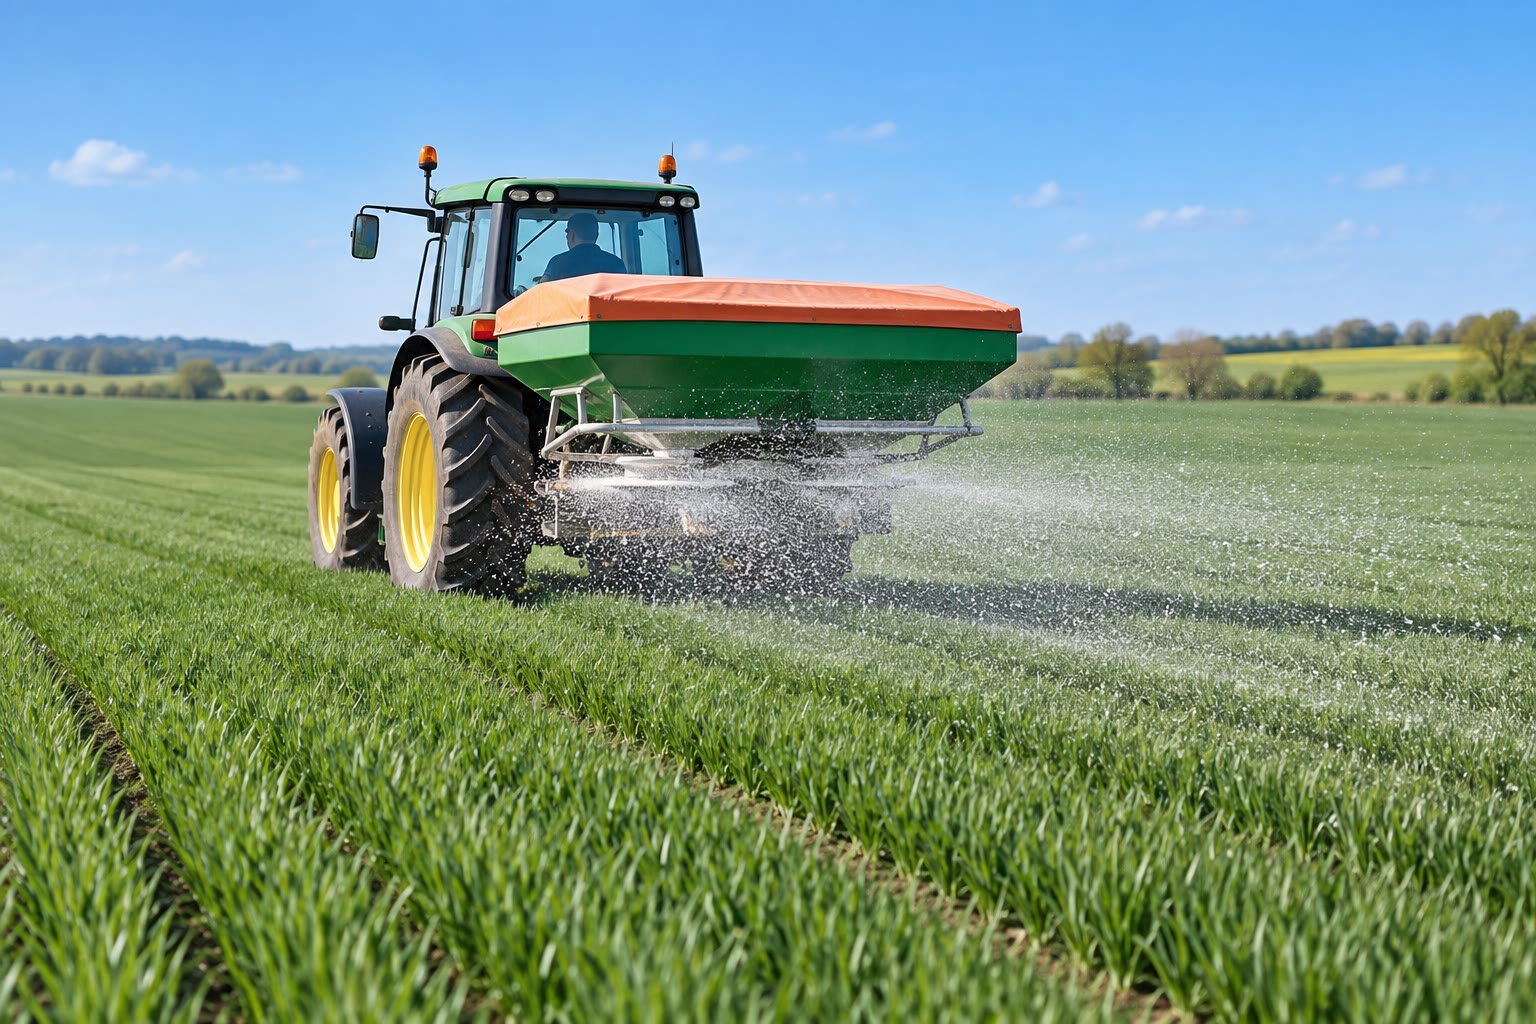
\includegraphics[width=0.55\linewidth]{images/book2/ai/b1-27-fertiliser-field.jpg}

{\small Aplicación de un fertilizante nitrogenado en un campo de trigo. La
mayor parte se fabricó a partir del nitrógeno del aire por el proceso
Haber--Bosch.}
\end{omfigure}

\section{El grupo 13: el boro y el aluminio}

El boro es un \omterm{def:b1:periodicity:metalloid}{metaloide} que forma compuestos covalentes con el octeto
incompleto: en \ce{BF3} y en el ácido bórico \ce{B(OH)3}, el boro tiene
seis \omterm{def:b1:quantum-numbers:configuration}{electrones de valencia} y actúa como \omterm{def:b1:lewis-resonance-vsepr:lewis-acid}{ácido de Lewis}
(\cref{ch:b1:lewis-resonance-vsepr}). El ácido bórico es un \omterm{def:b1:predominant-reaction:strong-acid}{ácido débil},
no porque pierda un protón, sino porque acepta un ion hidróxido,
\ce{B(OH)3 + 2H2O <=> B(OH)4- + H3O+}. El bórax, un borato de sodio, se
usa en el vidrio y en los detergentes.

\begin{definition}[Oxoácido]\label{def:b1:p-block-13-15:oxoacid}
Un \emph{oxoácido}\index{oxoacido@oxoácido} es un ácido cuyos átomos de
hidrógeno ácidos están unidos a átomos de oxígeno, a su vez unidos a un
\omterm{def:b1:complexation:complex}{átomo central}:
\ce{B(OH)3}, \ce{H2CO3}, \ce{HNO3} (\ce{HO-NO2}), \ce{H3PO4}
(\ce{(HO)3PO}), \ce{H2SO4}. Cuantos más átomos de oxígeno sin hidrógeno
rodean al \omterm{def:b1:complexation:complex}{átomo central}, más fuerte es el ácido.
\end{definition}

El aluminio, debajo del boro, es un metal, pero su ion pequeño y muy
cargado le da un óxido y un \omterm{def:b1:precipitation:amphoteric-hydroxide}{hidróxido anfóteros}
(\cref{sec:b1:precipitation:amphoteric}). Su mena es la bauxita, una
mezcla de hidróxidos de aluminio con óxidos de hierro y sílice; en 2025
el mundo extrajo unos 440 millones de toneladas de bauxita y refinó a
partir de ella unos 150 millones de toneladas de alúmina.
% ledger: usgs:bauxite-world-2025, usgs:alumina-world-2025

\begin{proposition}[El proceso Bayer]\label{prop:b1:p-block-13-15:bayer}
El hidróxido de sodio concentrado y caliente disuelve el aluminio de la
bauxita como \ce{Al(OH)4-} y deja los óxidos de hierro (lodo rojo); al
enfriar y sembrar la disolución filtrada precipita \ce{Al(OH)3} puro, que
se calcina a alúmina,
\ce{2Al(OH)3 -> Al2O3 + 3H2O}.
\end{proposition}

\begin{proof}
\ce{Al(OH)3(s) + OH- <=> Al(OH)4-} tiene $K = 10^{-1.23}$ a
\qty{25}{\celsius} (\cref{ch:b1:precipitation}): a \ce{[OH-]} alta, el
aluminio está en disolución, mientras que el hidróxido de hierro(III), que
no es anfótero, permanece sólido (\cref{exo:b1:precipitation:12}). La
dilución y el enfriamiento disminuyen \ce{[OH-]} y desplazan el cociente
de modo que $Q > K$ para la reacción inversa: el hidróxido precipita. La
calcinación elimina el agua.
\end{proof}

La alúmina se reduce después a aluminio por electrólisis en criolita
fundida, una industria que se estudia en el volumen del segundo año.

\begin{omfigure}
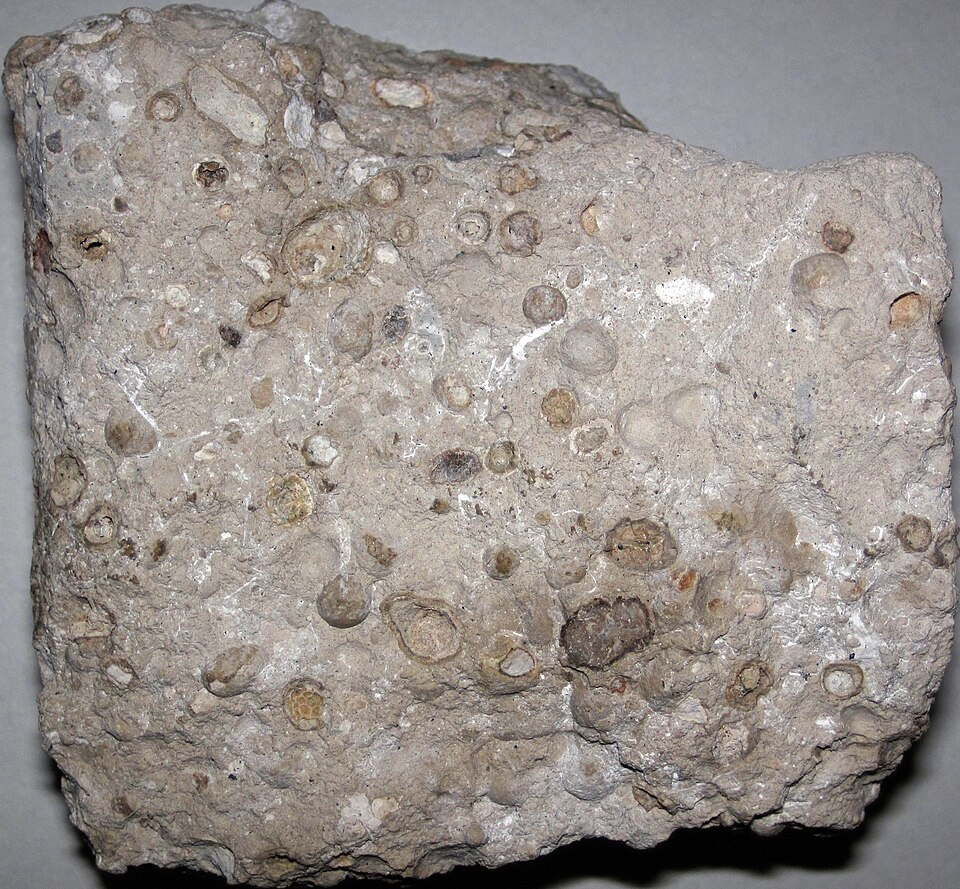
\includegraphics[height=3.6cm]{images/book2/bauxite.jpg}\hspace{0.4em}%
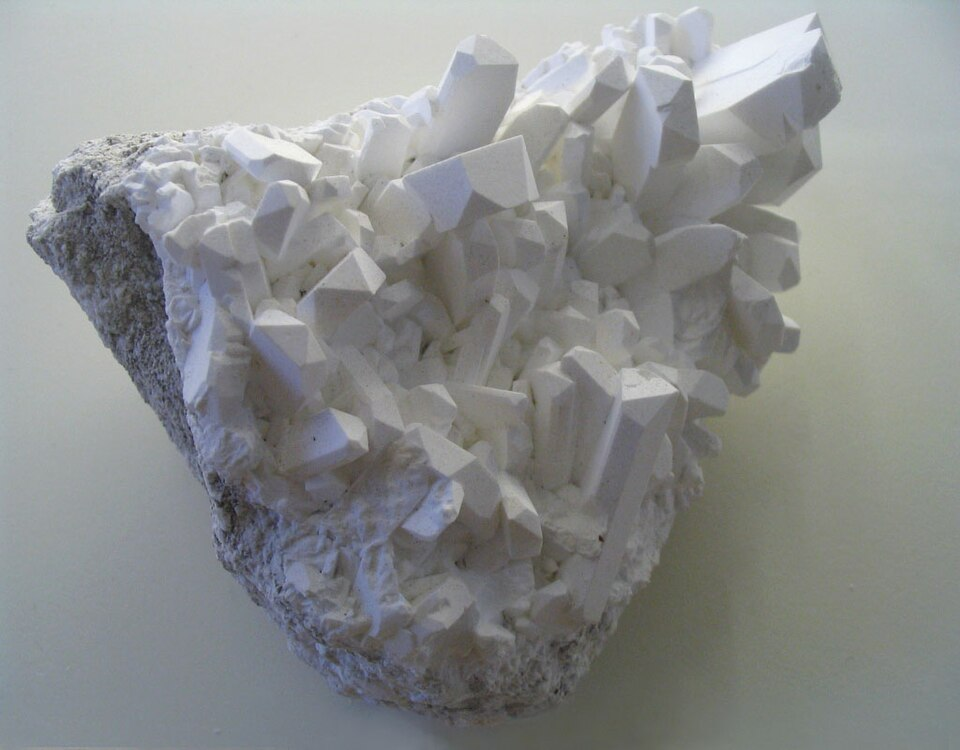
\includegraphics[height=3.6cm]{images/book2/borax.jpg}\hspace{0.4em}%
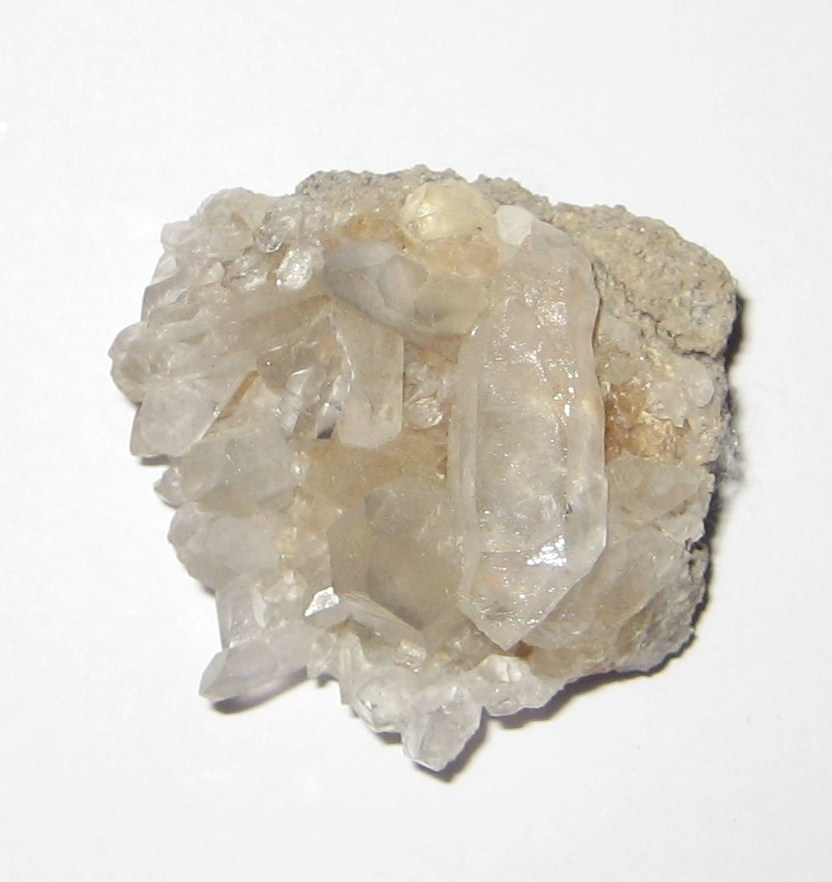
\includegraphics[height=3.6cm]{images/book2/quartz.jpg}\hspace{0.4em}%
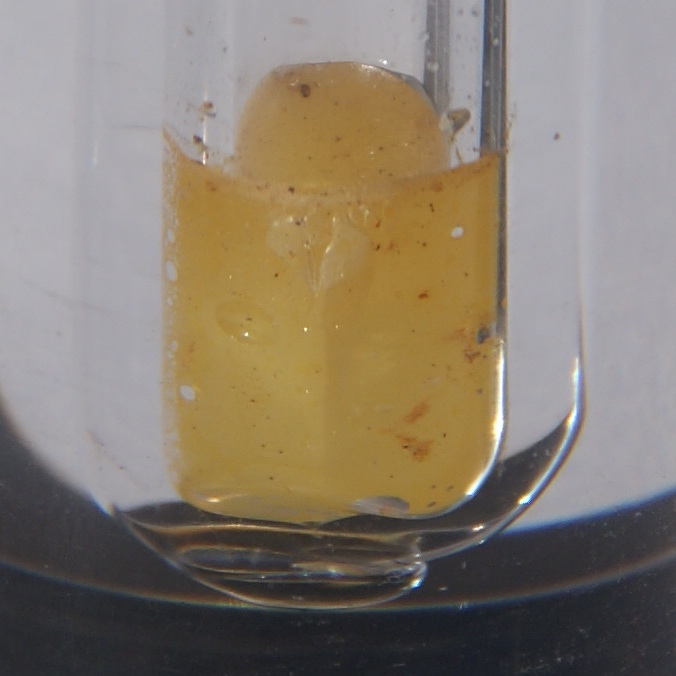
\includegraphics[height=3.6cm]{images/book2/white-phosphorus.jpg}

{\small De izquierda a derecha: bauxita pisolítica (James St. John, CC BY
2.0); \omterm{def:b1:crystals-metals:crystal}{cristales} de bórax (Aram Dulyan, dominio público); un racimo de
\omterm{def:b1:crystals-metals:crystal}{cristales} de cuarzo, \ce{SiO2} (Stephanie Clifford, CC BY 2.0); fósforo
blanco, con un poco de fósforo rojo, guardado bajo agua porque se inflama
en el aire (Hi-Res Images of Chemical Elements, CC BY 3.0). Todas de
Wikimedia Commons.}
\end{omfigure}

\section{El grupo 14: el carbono y el silicio}

El carbono y el silicio forman los dos cuatro enlaces, pero de manera
distinta. El carbono forma enlaces dobles fuertes: el \ce{CO2} es una
molécula, \ce{O=C=O}, un gas. El silicio apenas los forma: el \ce{SiO2}
es una red covalente de tetraedros \ce{SiO4} que comparten todos sus
vértices, un sólido duro, el cuarzo (\cref{ch:b1:crystals-ionic-covalent}).
El dióxido de carbono es un \omterm{def:b1:s-block:oxide-character}{óxido ácido}, que da ácido carbónico,
hidrogenocarbonatos y carbonatos (\cref{ch:b1:predominant-reaction}); la
sílice también es un \omterm{def:b1:s-block:oxide-character}{óxido ácido}, atacado por los álcalis fundidos para
dar silicatos.

\begin{proposition}[Unidades de silicato]\label{prop:b1:p-block-13-15:silicate-units}
Los silicatos están formados por tetraedros \ce{SiO4}; el número de
vértices compartidos con otros tetraedros fija la fórmula del anión:
ninguno, \ce{SiO4^4-} (tetraedros aislados); dos, cadenas
$(\ce{SiO3})_n^{2n-}$; tres, láminas $(\ce{Si2O5})_n^{2n-}$; cuatro, el
armazón neutro \ce{SiO2}.
\end{proposition}

\begin{proof}
Un oxígeno compartido pertenece a medias a cada tetraedro. Un tetraedro
que comparte $k$ vértices posee $4 - k$ átomos de oxígeno enteros y $k$ a
medias: $4 -
k/2$ oxígenos por silicio. Cada oxígeno no compartido lleva
una carga $-1$ (tiene un solo enlace), y cada uno compartido, ninguna: la
carga por silicio es $-(4 - k)$. $k = 0$: \ce{SiO4^4-}; $k = 2$:
\ce{SiO3^2-} por silicio; $k = 3$: \ce{SiO_{2.5}^-}, es decir,
\ce{Si2O5^2-}; $k = 4$: \ce{SiO2}.
\end{proof}

\begin{omfigure}
\begin{tikzpicture}[font=\small, line join=round]
  % one SiO4 tetrahedron in perspective
  \begin{scope}
    \coordinate (t) at (0,1.2); \coordinate (a) at (-1.0,-0.5);
    \coordinate (b) at (1.0,-0.5); \coordinate (c) at (0.25,0.05);
    \draw[thick, omDef] (t) -- (a) -- (b) -- cycle; \draw[thick, omDef] (t) -- (b);
    \draw[dashed, omDef] (a) -- (c) -- (b) (t) -- (c);
    \foreach \p in {t,a,b,c} \shade[ball color=red!60] (\p) circle (0.16);
    \shade[ball color=gray!40] (0.06,0.18) circle (0.11);
    \node at (0,-1.2) {\ce{SiO4^4-}: un tetraedro};
  \end{scope}
  % a chain of tetrahedra seen from above
  \begin{scope}[xshift=3.6cm]
    \foreach \i in {0,1,2,3} {
      \draw[thick, omDef, fill=omDef!10] (\i*1.1,0) -- (\i*1.1+0.55,0.95) -- (\i*1.1+1.1,0) -- cycle;
      \shade[ball color=red!60] (\i*1.1+0.55,0.95) circle (0.12);
      \shade[ball color=red!60] (\i*1.1+0.55,0.32) circle (0.10);
    }
    \foreach \i in {0,1,2,3,4} \shade[ball color=red!60] (\i*1.1,0) circle (0.12);
    \node[align=center] at (2.2,-1.0) {cadena $(\ce{SiO3})_n^{2n-}$: cada tetraedro\\ comparte dos vértices (vista desde arriba)};
  \end{scope}
\end{tikzpicture}

{\small Unidades de silicato: un tetraedro \ce{SiO4} aislado (silicio en
gris, oxígeno en rojo) y una cadena en la que cada tetraedro comparte dos
átomos de oxígeno con sus vecinos. Las láminas (tres vértices
compartidos) forman las micas y las arcillas; un armazón (cuatro), el
cuarzo.}
\end{omfigure}

\begin{definition}[Efecto del par inerte]\label{def:b1:p-block-13-15:inert-pair}
El \emph{efecto del par inerte}\index{efecto del par inerte} es la
estabilidad creciente, al descender por los \omterm{def:b1:periodicity:table}{grupos} 13 a 15, del estado
de oxidación dos unidades por debajo del máximo del grupo: talio(I) antes
que (III), plomo(II) antes que (IV), bismuto(III) antes que (V). El par
\textit{ns}$^2$ de los elementos pesados está fuertemente retenido y
apenas participa en el enlace.
\end{definition}

Este efecto explica por qué el óxido de plomo(IV) es un \omterm{def:b1:nernst:couple}{oxidante} fuerte
($E^\circ(\ce{PbO2}/\ce{Pb^2+}) = 1.46$~V, \cref{ch:b1:nernst}), mientras
que el carbono(IV) y el silicio(IV) son los estados estables de sus
elementos.

\section{El grupo 15: el nitrógeno}

\begin{proposition}[La escala del nitrógeno]\label{prop:b1:p-block-13-15:nitrogen-ladder}
El nitrógeno adopta todos los \omterm{def:b1:nernst:oxidation-number}{números de oxidación} de $-3$ a $+5$:
\ce{NH3} y \ce{NH4+} ($-$III), \ce{N2H4} ($-$II), \ce{NH2OH} ($-$I),
\ce{N2} (0), \ce{N2O} ($+$I), \ce{NO} ($+$II), \ce{HNO2} y \ce{NO2-}
($+$III), \ce{NO2} ($+$IV), \ce{HNO3} y \ce{NO3-} ($+$V).
\end{proposition}

\begin{proof}
Se aplican las reglas de la \cref{prop:b1:nernst:on-rules} a cada
fórmula, con H en $+$I y O en $-$II: en \ce{N2H4}, $2x + 4 = 0$; en
\ce{NO2-}, $x - 4 =
-1$; y así sucesivamente.
\end{proof}

\begin{definition}[Fijación del nitrógeno]\label{def:b1:p-block-13-15:nitrogen-fixation}
La \emph{fijación del nitrógeno}\index{fijacion del nitrogeno@fijación del nitrógeno} es cualquier proceso
que convierte el dinitrógeno del aire en un compuesto (amoniaco, nitrato)
que los seres vivos o la industria pueden usar: la fijación biológica
por bacterias, la fijación por los rayos y la síntesis industrial del
amoniaco.
\end{definition}

El proceso Haber--Bosch combina nitrógeno e hidrógeno sobre un
\omterm{def:b1:elementary-steps:catalyst}{catalizador} de hierro, \ce{N2 + 3H2 <=> 2NH3}. La reacción está
favorecida a temperatura ambiente ($K = 10^{5.8}$ a \qty{25}{\celsius},
a partir de la energía de Gibbs de formación del amoniaco), pero es
demasiado lenta; el \omterm{def:b1:elementary-steps:catalyst}{catalizador} solo funciona en caliente, y la elección
de la temperatura y la presión que concilia velocidad y \omterm{def:b1:extent-q-and-k:fractional-extent}{rendimiento} se
hace en el volumen del segundo año. El amoniaco se oxida después a ácido
nítrico por el proceso Ostwald.
% ledger: dfg:NH3_g

\begin{omfigure}
\begin{tikzpicture}[font=\small, >={Stealth}, box/.style={draw, rounded corners, fill=omDef!8, align=center, minimum height=0.9cm}]
  \node[box] (air) at (0,0) {aire\\\ce{N2}};
  \node[box] (gas) at (0,-1.6) {gas natural\\\ce{H2}};
  \node[box] (hb) at (3.4,-0.8) {Haber--Bosch\\catalizador\\de hierro};
  \node[box] (ox1) at (7.3,-0.8) {malla Pt--Rh\\\ce{NH3} $\to$ \ce{NO}};
  \node[box] (ox2) at (11.0,-0.8) {oxidación\\absorción\\\ce{NO} $\to$ \ce{NO2} $\to$ \ce{HNO3}};
  \draw[->, thick] (air) -- (hb);
  \draw[->, thick] (gas) -- (hb);
  \draw[->, thick] (hb) -- node[above] {\ce{NH3}} (ox1);
  \draw[->, thick] (ox1) -- node[above] {\ce{NO}} (ox2);
  \draw[->, thick] (ox2.south) -- ++(0,-0.6) node[below] {\ce{HNO3}};
  \draw[->, thick] (hb.south) -- ++(0,-0.9) node[below] {\ce{NH3} (fertilizantes)};
  \draw[->, thick] (ox2.north) -- ++(0,0.5) -| node[pos=0.25, above] {\ce{NO} reciclado} (ox1.north);
\end{tikzpicture}

{\small Del aire al ácido nítrico: la síntesis del amoniaco seguida de las
tres etapas del proceso Ostwald.}
\end{omfigure}

\begin{method}[Ajustar ecuaciones industriales encadenadas]\label{met:b1:p-block-13-15:ostwald-balance}
\begin{enumerate}
  \item Se ajusta cada etapa: (1) \ce{4NH3 + 5O2 -> 4NO + 6H2O};
        (2) \ce{2NO + O2 -> 2NO2}; (3) \ce{3NO2 + H2O -> 2HNO3 + NO}.
  \item Se multiplican las etapas de modo que cada intermedio formado se
        consuma (el \ce{NO} de la etapa 3 vuelve a la etapa 2).
  \item Se suman: con reciclado completo del NO, la ecuación global es
        \ce{NH3 + 2O2 -> HNO3 + H2O}, un ácido nítrico por cada amoniaco.
  \item Se usa la ecuación global para los balances de materia, y las
        etapas para el diseño de cada reactor.
\end{enumerate}
\end{method}

\begin{history}[Fritz Haber]
\begin{minipage}[t]{0.18\linewidth}\vspace{0pt}
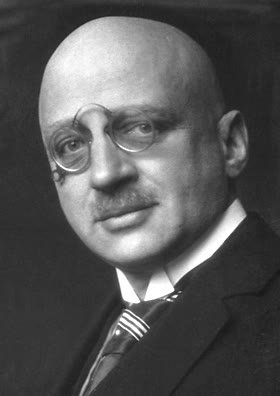
\includegraphics[width=\linewidth]{images/book2/haber.jpg}
\end{minipage}\hfill
\begin{minipage}[t]{0.78\linewidth}\vspace{0pt}
Fritz Haber demostró que el amoniaco podía obtenerse a partir de
nitrógeno e hidrógeno a presión sobre un \omterm{def:b1:elementary-steps:catalyst}{catalizador}; Carl Bosch
convirtió la reacción de laboratorio en un proceso industrial. Haber
recibió el Premio Nobel de Química de 1918. El mismo hombre dirigió el
primer uso a gran escala del cloro como arma en la Primera Guerra
Mundial: la química que alimenta a media humanidad y la química que mata
están separadas por las decisiones de los químicos. (Fotografía: The
Nobel Foundation, publicada en 1919, dominio público, Wikimedia Commons.)
\end{minipage}
\end{history}

\section{El fósforo y las tendencias a lo largo de los grupos}

El fósforo, debajo del nitrógeno, no forma enlaces triples \ce{P#P}: el
fósforo blanco está formado por tetraedros \ce{P4}, tensionados y
reactivos (se inflama en el aire y se guarda bajo agua); el fósforo rojo
es un polímero, mucho menos reactivo. La combustión del fósforo da
\ce{P4O10}, el más ácido de los óxidos comunes, que con agua da ácido
fosfórico,
$\mathrm{p}K_a$ 2.15, 7.21, 12.34 (\cref{ch:b1:predominant-reaction}).
La roca fosfática, de la que se extrajeron unos 250 millones de toneladas
en 2025, se transforma con ácido sulfúrico en fertilizantes fosfatados.
% ledger: usgs:phosphate-world-2025

Al descender por cada grupo, los elementos se vuelven más metálicos (del
boro al talio, del carbono al plomo, del nitrógeno al bismuto), sus
óxidos más básicos, y los estados de oxidación más bajos más estables: el
\omterm{def:b1:p-block-13-15:inert-pair}{efecto del par inerte}. A lo largo de un \omterm{def:b1:periodicity:table}{periodo}, los óxidos se vuelven
más ácidos, desde el \ce{Na2O} básico hasta los \omterm{def:b1:s-block:oxide-character}{óxidos ácidos} del fósforo
y del azufre.

\section{Ejercicios}

\begin{exercise}[$\star$]\label{exo:b1:p-block-13-15:1}
Dese el \omterm{def:b1:nernst:oxidation-number}{número de oxidación} del nitrógeno en \ce{NH4NO3} (los dos
átomos), \ce{N2O5}, \ce{HNO2}, \ce{N2H4} y \ce{Mg3N2}.
\end{exercise}

\begin{exercise}[$\star$]\label{exo:b1:p-block-13-15:2}
Dibújense las \omterm{def:b1:lewis-resonance-vsepr:lewis}{estructuras de Lewis} de \ce{BF3}, de \ce{NH3} y del aducto
\ce{F3B-NH3}; identifíquense el ácido y la \omterm{def:b1:lewis-resonance-vsepr:lewis-acid}{base de Lewis}.
\end{exercise}

\begin{exercise}[$\star$]\label{exo:b1:p-block-13-15:3}
Escríbanse las reacciones del \ce{CO2}, del \ce{SiO2} (fundido) y del
\ce{P4O10} con el hidróxido de sodio, y las del \ce{Al2O3} con un ácido y
con una base.
\end{exercise}

\begin{exercise}[$\star$]\label{exo:b1:p-block-13-15:4}
Calcúlese la constante de equilibrio de \ce{N2 + 3H2 <=> 2NH3} a
\qty{25}{\celsius} a partir de $\Delta_f G^\circ(\ce{NH3}) =
\qty{-16.45}{kJ/mol}$.
\end{exercise}

\begin{exercise}[$\star\star$]\label{exo:b1:p-block-13-15:5}
Con el recuento de la \cref{prop:b1:p-block-13-15:silicate-units}, dese
la fórmula de un anillo de seis tetraedros que comparten cada uno dos
vértices (como en el berilo) y la de una cadena doble en la que la mitad
de los tetraedros comparten dos vértices y la otra mitad, tres.
\end{exercise}

\begin{exercise}[$\star\star$]\label{exo:b1:p-block-13-15:6}
Calcúlese la masa de alúmina obtenida a partir de una tonelada de
bauxita que contiene un \qty{55}{\percent} en masa de \ce{Al(OH)3}, con
una recuperación del \qty{92}{\percent}.
\end{exercise}

\begin{exercise}[$\star\star$]\label{exo:b1:p-block-13-15:7}
Demuéstrese que el ácido bórico es un \omterm{def:b1:lewis-resonance-vsepr:lewis-acid}{ácido de Lewis} y no de Brønsted, y
explíquese por qué su disolución es, sin embargo, ácida.
\end{exercise}

\begin{exercise}[$\star\star$]\label{exo:b1:p-block-13-15:8}
Ajústese con los \omterm{def:b1:nernst:oxidation-number}{números de oxidación} la oxidación del amoniaco a
\ce{NO}, y dese el número de electrones intercambiados por cada \ce{NH3}.
\end{exercise}

\begin{exercise}[$\star\star$]\label{exo:b1:p-block-13-15:9}
El nitrato de amonio se fabrica a partir de amoniaco y ácido nítrico.
Escríbase la reacción y calcúlese la masa de amoniaco necesaria (tanto
para el ácido nítrico como para la neutralización) por tonelada de
nitrato de amonio.
\end{exercise}

\begin{exercise}[$\star\star\star$]\label{exo:b1:p-block-13-15:10}
Explíquese por qué el nitrógeno es un gas diatómico y el fósforo un
sólido de moléculas \ce{P4}, y por qué el dióxido de carbono es un gas y
la sílice un sólido, a partir de la fuerza de los enlaces $\pi$ entre
átomos del segundo y del tercer \omterm{def:b1:periodicity:table}{periodo}.
\end{exercise}

\begin{exercise}[$\star\star\star$]\label{exo:b1:p-block-13-15:11}
Demuéstrese con los \omterm{def:b1:nernst:electrode-potential}{potenciales estándar} que el óxido de plomo(IV) oxida
los iones cloruro a cloro en medio ácido, mientras que el óxido de
silicio(IV) no hace nada parecido. Relaciónese con el \omterm{def:b1:p-block-13-15:inert-pair}{efecto del par
inerte}.
\end{exercise}

\begin{exercise}[$\star\star\star$]\label{exo:b1:p-block-13-15:12}
El mundo produjo unos 160 millones de toneladas de nitrógeno en forma de
amoniaco en 2025. ¿Qué masa de amoniaco representa, y qué masa de
hidrógeno contenía? ¿De dónde procede sobre todo ese hidrógeno?
\end{exercise}

\section{Problema: del aire al fertilizante}

\begin{problem}[{Problema de fin de semana --- el enlace triple del
nitrógeno, la síntesis del amoniaco, las tres etapas de la fabricación
del ácido nítrico, el nitrato de amonio, y la masa de ácido nítrico que
puede obtenerse de una tonelada de amoniaco}]
\label{pb:b1:p-block-13-15:1}
Una planta de fertilizantes convierte el amoniaco en ácido nítrico y en
nitrato de amonio. Masas molares (\unit{g/mol}): \ce{N2} 28.0, \ce{H2}
2.0, \ce{NH3}
17.0, \ce{HNO3} 63.0, \ce{NH4NO3} 80.0, \ce{O2} 32.0;
$\Delta_f G^\circ(\ce{NH3(g)}) = \qty{-16.45}{kJ/mol}$ a
\qty{25}{\celsius}.

\medskip
\noindent\textbf{Parte I --- El nitrógeno.}
\begin{enumerate}
  \item Dibújese la \omterm{def:b1:lewis-resonance-vsepr:lewis}{estructura de Lewis} del \ce{N2} y dígase por qué es
        poco reactivo.
  \item Dese el \omterm{def:b1:nernst:oxidation-number}{número de oxidación} del N en \ce{N2}, \ce{NH3}, \ce{NO},
        \ce{NO2}, \ce{HNO3} y \ce{NH4NO3}.
  \item Nómbrense tres formas, naturales o industriales, de fijar el
        nitrógeno.
  \item ¿Por qué las plantas no pueden usar directamente el \ce{N2}?
  \item ¿Qué elemento se oxida y cuál se reduce en la síntesis del
        amoniaco?
  \item Escríbase la síntesis del amoniaco.
\end{enumerate}

\medskip
\noindent\textbf{Parte II --- El amoniaco.}
\begin{enumerate}[resume]
  \item Calcúlese la constante de equilibrio de la síntesis a
        \qty{25}{\celsius}.
  \item ¿Por qué se lleva a cabo, sin embargo, la síntesis en caliente y
        sobre un \omterm{def:b1:elementary-steps:catalyst}{catalizador}?
  \item Calcúlense las masas de \ce{N2} y de \ce{H2} para una tonelada de
        amoniaco.
  \item ¿Qué volumen de aire (\qty{78}{\percent} de \ce{N2} en volumen,
        gas ideal, \qty{25}{\celsius}, \qty{1}{bar}) contiene ese
        nitrógeno?
  \item ¿De dónde procede el hidrógeno?
  \item ¿Por qué en algunos países se usa el propio amoniaco como
        fertilizante, y por qué a menudo se transforma antes?
\end{enumerate}

\medskip
\noindent\textbf{Parte III --- El ácido nítrico.}
\begin{enumerate}[resume]
  \item Ajústese la etapa 1, \ce{NH3 + O2 -> NO + H2O}, con los \omterm{def:b1:nernst:oxidation-number}{números de oxidación}. % ce-unbalanced-ok
  \item Ajústese la etapa 2, \ce{NO + O2 -> NO2}. % ce-unbalanced-ok
  \item Ajústese la etapa 3, \ce{NO2 + H2O -> HNO3 + NO}. ¿Qué tipo de % ce-unbalanced-ok
        reacción redox es?
  \item Combínense las etapas, con reciclado completo del NO, en la
        ecuación global.
  \item Calcúlese la masa de oxígeno consumida por tonelada de amoniaco.
  \item ¿Por qué se usa una malla de platino--rodio en la etapa 1?
\end{enumerate}

\medskip
\noindent\textbf{Parte IV --- El nitrato de amonio y los balances de materia.}
\begin{enumerate}[resume]
  \item Escríbase la formación del nitrato de amonio.
  \item ¿Qué fracción del amoniaco debe transformarse en ácido nítrico
        para fabricar solo nitrato de amonio?
  \item Calcúlese la masa de nitrato de amonio obtenida de una tonelada de
        amoniaco repartida de ese modo.
  \item ¿Qué porcentaje de nitrógeno contiene el nitrato de amonio?
  \item ¿Por qué debe almacenarse el nitrato de amonio lejos de los
        combustibles y del calor?
  \item Calcúlese la masa de ácido nítrico que puede obtenerse de una
        tonelada de amoniaco (conversión completa).
\end{enumerate}
\end{problem}
